\section{Privacy}
\subsection*{Privacy Attacks}
\begin{itemize}
    \item Model stealing (white/black box)
    \item Model inversion: Client queries the model to find representative samples.
    \item Data extraction: Client queries the model to find exact training samples.
    \item Membership inference: Client wants to determine if the data
          point was used to train the model or not (train shadow models)
\end{itemize}

\subsection*{Differential Privacy}
A randomized algorithm $M$ is $\epsilon, \delta$-DP if for all "neighbouring" \ datasets $D, D^\prime$ and all sets (attacks) $S$,
$$\P\left[M(D)\in S\right] \le e^\epsilon \P\left[M(D^\prime)\in S\right]+\delta.$$
\vspace*{-4mm}
\subsection*{DP Rules}
Post-processing: If $M$ is $\epsilon,\delta$-DP, then $g\circ M$ is $\epsilon,\delta$-DP.\\
Composition: If $M_1,M_2$ are $\varepsilon_1,\delta_1$-DP and $\varepsilon_2,\delta_2$-DP, then $M:=(M_1,M_2)$ is $(\varepsilon_1+\varepsilon_2,\delta_1+\delta_2)$-DP.\\
Privacy Amplification: Applying an $\epsilon,\delta$-DP mechanism on a random fraction $q\leq1$ subset yields a $\tilde{q}\epsilon,q\delta$-DP mechanism, where $\tilde{q}\approx q$.\\
If there is a pair $(D,D')\in \mathrm{Neigh}$ and a set $S$ s.t. $\P[M(D)\in S]>0=\P[M(D')\in S]$, then $M$ is not $\varepsilon$-DP for any $\varepsilon$.

\subsection*{Laplace Mechanism}
Let $\Delta_1=\max_{D\sim_{\text{neigh}}D'}\|f(D)-f(D')\|_{1}$. Then $f+\text{Laplace}(0,\Delta_1/\epsilon)$ is $\varepsilon$-DP.\\
Density: $\frac{1}{2\sigma}e^{-\frac{|x-\mu|}{\sigma}}$

\subsection*{Gaussian Mechanism}
Let $\Delta_2=\max_{D\sim_{\text{neigh}}D'}\|f(D)-f(D')\|_{{2}}$. Then if $\sigma^2=\frac{2\log(1.25)}{\delta\epsilon^2}\Delta_2^2$ we get that $f+\No(0,\sigma^2I)$ is $\varepsilon,\delta$-DP.
Density: $({{2\pi\sigma^2}})^{-1/2}e^{-\frac{(x-\mu)^2}{2\sigma^2}}$

\subsection*{DP-SGD}
$\varepsilon,\delta$-DP adaptation of SGD.
\begin{enumerate}
    \item Clip gradients: ${g}'_i=\min\left(\frac{R}{\|{g}\|_2},1\right){g_i}$
    \item Aggregate: $\bar{g}=\frac{1}{n}\sum_{i=1}^n {g}'_i$
    \item Add noise: $\tilde{g}=\bar{g}+\No(0,\sigma^2I)$ where $\sigma^2=\frac{2\log(1.25)}{\delta \epsilon^2}\frac{R^2}{n^2}$
    \item Update: $\theta\leftarrow \theta-\eta\tilde{g}$
\end{enumerate}
DP-SGD is $O\left(q\varepsilon\sqrt{T\log{\frac{1}{\delta}}}\right),O(qT\delta)$-DP. It is $O(q\varepsilon\sqrt{T}),\delta$-DP when allowing data-dependent $\sigma$.

\subsection*{PATE}
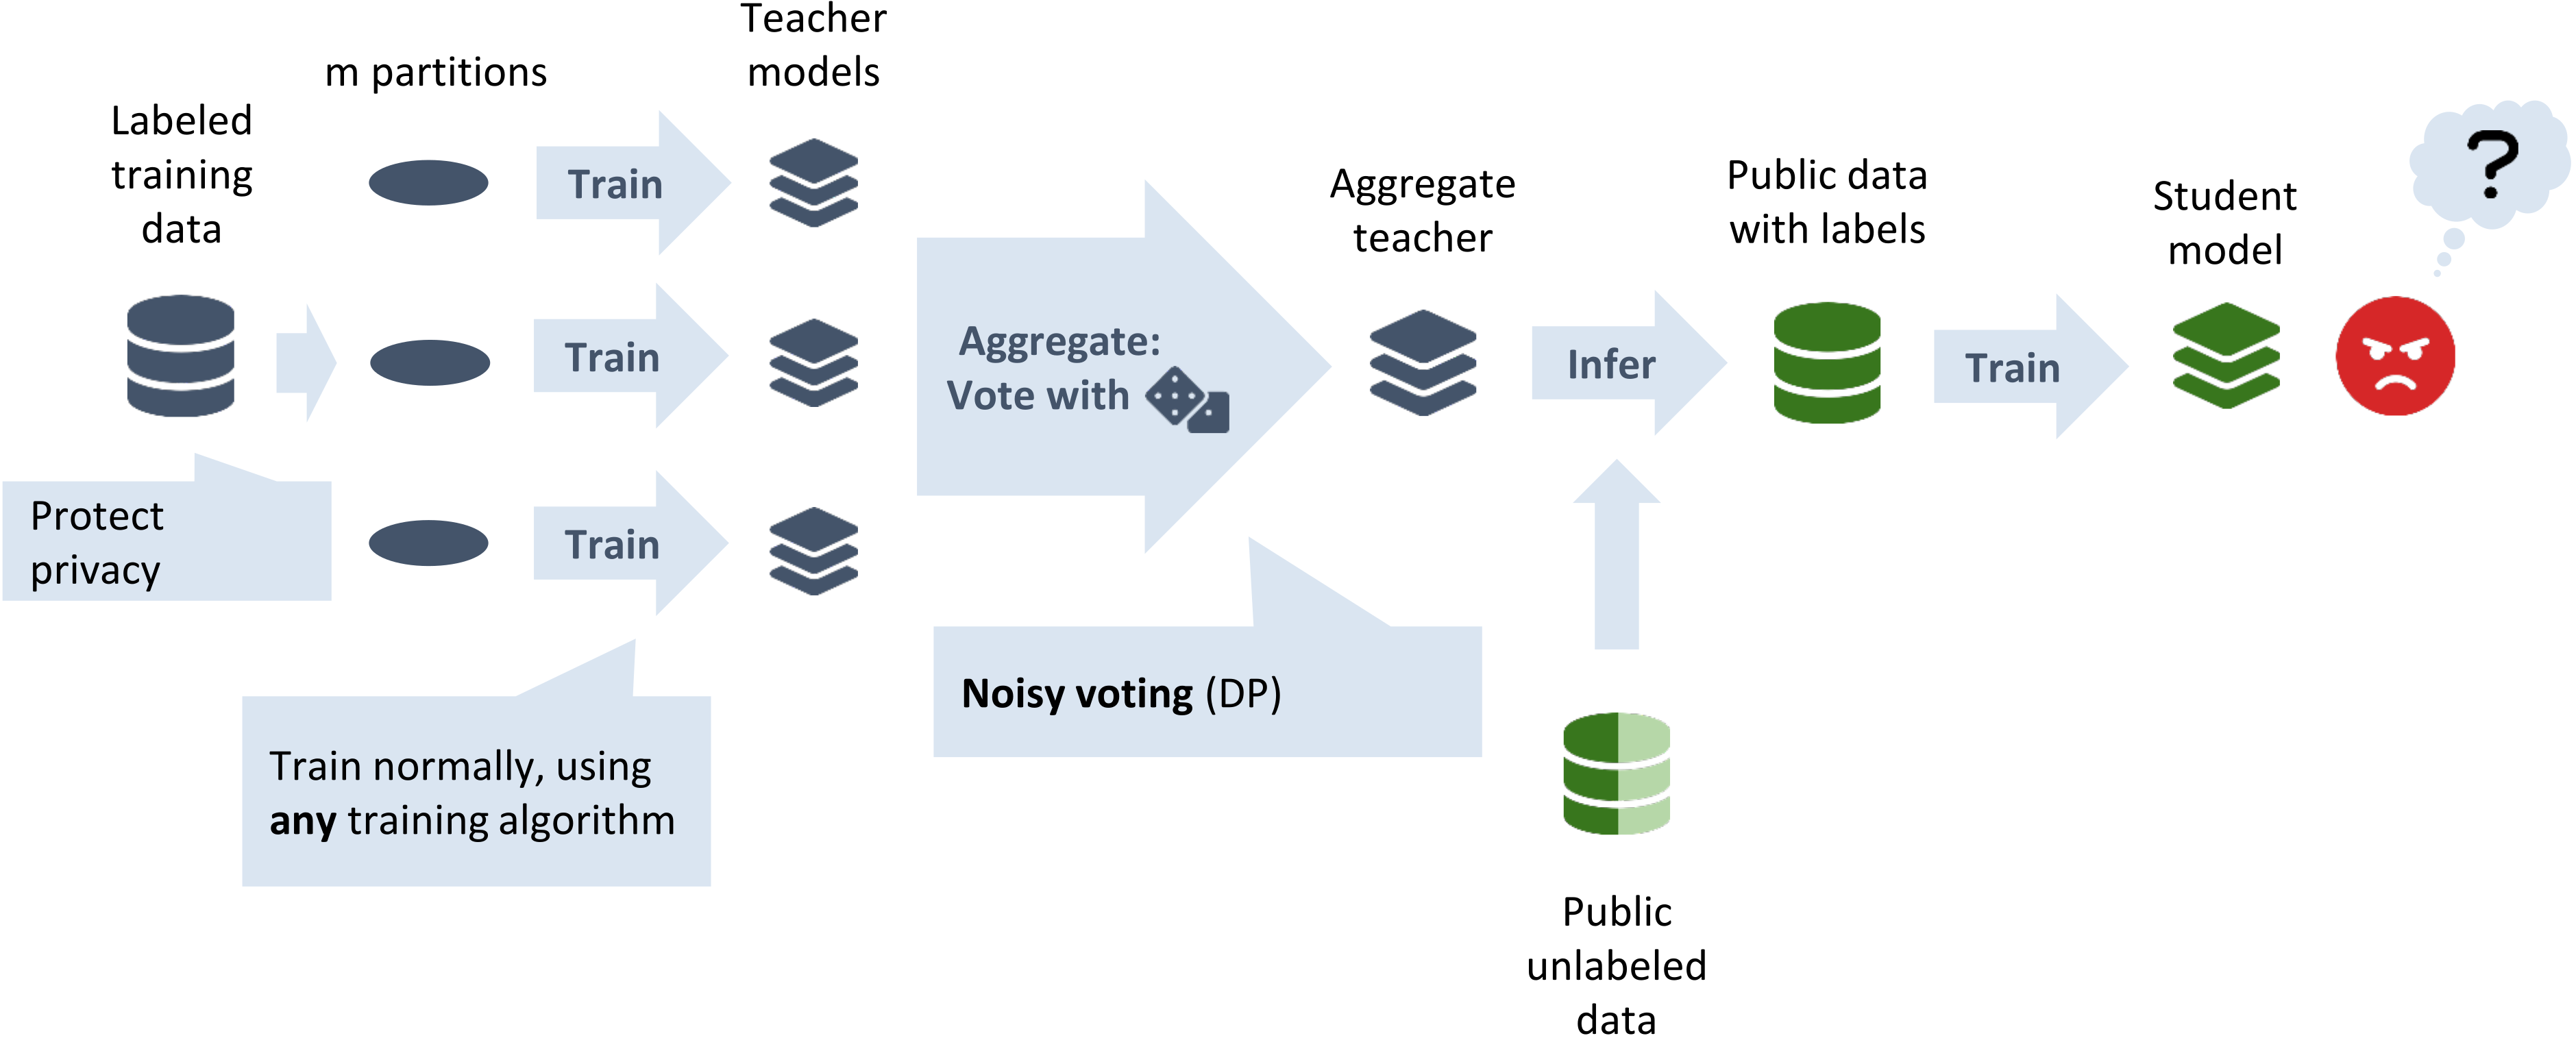
\includegraphics[width=\columnwidth]{img/pate.png}
Noisy voting: Add $\text{Laplace}(0,\frac{2}{\varepsilon})$-noise to each class count $n_c(x)$ before $\argmax$ ($n_c$ has $L_1$-sensitivity 2). Results in $N\varepsilon$-DP, where $N$ is the number of classifications we compute on the public unlabeled data.
